\documentclass[11pt]{beamer}

% --- Theme and Packages ---
\usetheme{Madrid}
\usecolortheme{default}
\usepackage[utf8]{inputenc}
\usepackage[T1]{fontenc}
\usepackage{graphicx}
\usepackage{booktabs}
\usepackage{hyperref}
\usepackage{tikz}
\usetikzlibrary{shapes.geometric, arrows.meta, positioning, fit}

% --- Title Information ---
\title[Helpful Community Notes]{Predicting Helpful Community Notes with Prompting and Parameter-Efficient Fine-Tuning}
\subtitle{Final Project Presentation}
\author[Madan, Pashkov, Salim]{Mridul Madan (01667156) \and Rafael Pashkov (02183763) \and Md Shahidul Salim (02207019)}
\institute[UMass Lowell]{University of Massachusetts Lowell}
\date{Social Computing Final Presentation}

\begin{document}
	
	% --- Slide 1: Title ---
	\begin{frame}
		\titlepage
	\end{frame}
	
	% --- Slide 2: Motivation ---
	\begin{frame}
		\frametitle{Motivation and Research Question}
		\begin{itemize}
			\item Online misinformation spreads faster than expert fact-checking can respond.
			\item Twitter/X \textbf{Community Notes} is a crowd-sourced fact-checking system where notes are shown only if raters from diverse viewpoints judge them helpful.
			\item Prior work mostly studies the \textit{rating system} or platform impact.
			\item Our focus is a \textbf{content-based prediction task}: can we predict note helpfulness from the note text itself?
		\end{itemize}
		
		\vspace{0.4cm}
		\textbf{Research Question:} Which approach works best for this task:
		\begin{itemize}
			\item prompting,
			\item a supervised BERT baseline, or
			\item parameter-efficient fine-tuning with LoRA?
		\end{itemize}
	\end{frame}
	
	% --- Slide 3: What We Completed ---
	\begin{frame}
		\frametitle{What We Completed}
		\begin{itemize}
			\item Built a binary classification benchmark from public Community Notes data.
			\item Evaluated \textbf{Gemma-3-4B-IT} and \textbf{Qwen3-4B-Instruct} with:
			\begin{itemize}
				\item zero-shot prompting,
				\item few-shot prompting,
				\item chain-of-thought prompting,
				\item LoRA fine-tuning.
			\end{itemize}
			\item Implemented a supervised \textbf{BERT-base-uncased} baseline.
			\item Used the same temporal train/test split across all experiments.
			\item Compared models using accuracy, precision, recall, and F1.
		\end{itemize}
	\end{frame}
	
	% --- Slide 4: Dataset and Task ---
	\begin{frame}
		\frametitle{Dataset and Task}
		\begin{itemize}
			\item \textbf{Source:} Public Twitter/X Community Notes dataset.
			\item \textbf{Task:} Predict whether a note is \texttt{CURRENTLY\_RATED\_HELPFUL}.
			\item Excluded notes labeled \texttt{NEEDS\_MORE\_RATINGS}.
			\item Temporal split with zero overlap between train and test notes.
		\end{itemize}
		
		\vspace{0.2cm}
		\begin{table}
			\centering
			\small
			\begin{tabular}{lcc}
				\toprule
				\textbf{Statistic} & \textbf{Train} & \textbf{Test} \\
				\midrule
				Notes & 754 & 246 \\
				Helpful (\%) & 49.7\% & 54.5\% \\
				Not Helpful (\%) & 50.3\% & 45.5\% \\
				Mean word count & 31.4 & 31.7 \\
				Median word count & 33 & 33 \\
				Mean ratings per note & 50.1 & 50.2 \\
				FK grade level & 11.2 & 11.0 \\
				Date range & Jan--Sep 2024 & Oct--Dec 2024 \\
				\bottomrule
			\end{tabular}
		\end{table}
		
		\vspace{0.1cm}
		\textbf{Why this split matters:} temporal separation reduces leakage and better simulates deployment on future notes.
	\end{frame}
	
	% --- Slide 5: Dataset Statistics ---
	\begin{frame}
		\frametitle{Dataset Statistics}
		\begin{columns}[T]
			\column{0.49\textwidth}
			\textbf{Overall shape}
			\begin{itemize}
				\item 1,000 total notes
				\item 509 Helpful (50.9\%)
				\item 491 Not Helpful (49.1\%)
				\item Date range: Jan 1 to Dec 29, 2024
				\item Ratings per note: mean 50.2, median 48.5
			\end{itemize}
			
			\column{0.49\textwidth}
			\textbf{Text characteristics}
			\begin{itemize}
				\item Mean note length: 31.4 words
				\item Range: 6 to 53 words
				\item Helpful notes are slightly longer: 32.7 vs 30.0 words
				\item Readability is nearly identical: 11.2 vs 11.1 FK grade
			\end{itemize}
		\end{columns}
		
		\vspace{0.3cm}
		\textbf{Takeaway:} the task is challenging because notes are short and class-balanced, so performance gains likely come from learning subtle linguistic patterns rather than exploiting obvious dataset skew.
	\end{frame}
	
	% --- Slide 6: Input and Output Example ---
	\begin{frame}
		\frametitle{Input and Output Example}
		\small
		\textbf{Original Post Context}
		
		``Education reforms have increased school performance by 30\% since implementation began last year.''
		
		\vspace{0.3cm}
		\begin{columns}[T]
			\column{0.48\textwidth}
			\textbf{Input Note A}
			
			``The claim about education reforms is misleading. The original tweet's figures are not consistent with publicly available data from authoritative sources. Specifically, the reported numbers decreased by 0.4\% in Q3 2024.''
			
			\vspace{0.3cm}
			\textbf{Model Output}
			
			\textcolor{green!50!black}{\texttt{HELPFUL}}
			
			\vspace{0.2cm}
			\textbf{Why:} specific correction, evidence-oriented wording, clear contradiction of the claim.
			
			\column{0.48\textwidth}
			\textbf{Input Note B}
			
			``The question of education reforms is complex. There are arguments on both sides of this issue. Some experts believe one way, while others disagree. More research is needed to reach a definitive conclusion.''
			
			\vspace{0.3cm}
			\textbf{Model Output}
			
			\textcolor{red!70!black}{\texttt{NOT\_HELPFUL}}
			
			\vspace{0.2cm}
			\textbf{Why:} vague, hedged, and provides no concrete evidence or correction.
		\end{columns}
	\end{frame}
	
	% --- Slide 7: Methodology ---
	\begin{frame}
		\frametitle{Methodology Overview}
		\begin{center}
			\resizebox{0.96\textwidth}{!}{
				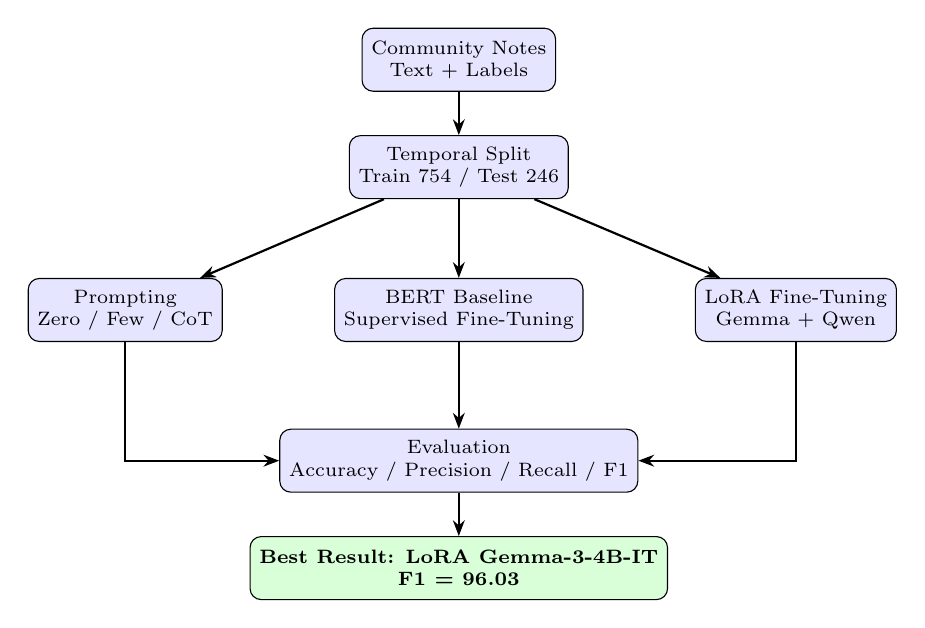
\begin{tikzpicture}[
					node distance=0.55cm and 0.8cm,
					box/.style={rectangle, rounded corners, minimum width=2.3cm, minimum height=0.8cm, align=center, draw=black, fill=blue!10, font=\scriptsize},
					highlight/.style={rectangle, rounded corners, minimum width=2.6cm, minimum height=0.8cm, align=center, draw=black, fill=green!15, font=\scriptsize\bfseries},
					arrow/.style={-{Stealth[length=2mm]}, thick}
					]
					\node (data) [box] {Community Notes\\Text + Labels};
					\node (split) [box, below=of data] {Temporal Split\\Train 754 / Test 246};
					
					\node (prompt) [box, below left=1.0cm and 1.6cm of split] {Prompting\\Zero / Few / CoT};
					\node (bert) [box, below=1.0cm of split] {BERT Baseline\\Supervised Fine-Tuning};
					\node (lora) [box, below right=1.0cm and 1.6cm of split] {LoRA Fine-Tuning\\Gemma + Qwen};
					
					\node (eval) [box, below=1.1cm of bert] {Evaluation\\Accuracy / Precision / Recall / F1};
					\node (best) [highlight, below=of eval] {Best Result: LoRA Gemma-3-4B-IT\\F1 = 96.03};
					
					\draw [arrow] (data) -- (split);
					\draw [arrow] (split) -- (prompt);
					\draw [arrow] (split) -- (bert);
					\draw [arrow] (split) -- (lora);
					\draw [arrow] (prompt) |- (eval);
					\draw [arrow] (bert) -- (eval);
					\draw [arrow] (lora) |- (eval);
					\draw [arrow] (eval) -- (best);
				\end{tikzpicture}
			}
		\end{center}
	\end{frame}
	
	% --- Slide 8: Prompting Results ---
	\begin{frame}
		\frametitle{Prompting Results}
		\begin{table}
			\centering
			\scriptsize
			\begin{tabular}{llcccc}
				\toprule
				\textbf{Strategy} & \textbf{Model} & \textbf{Acc} & \textbf{Prec} & \textbf{Rec} & \textbf{F1} \\
				\midrule
				Zero-shot & Gemma & 45.53 & 0.00 & 0.00 & 0.00 \\
				Zero-shot & Qwen & 45.53 & 0.00 & 0.00 & 0.00 \\
				Few-shot & Gemma & 52.44 & 56.69 & 53.73 & 55.17 \\
				Few-shot & Qwen & 49.19 & 53.19 & 55.97 & 54.55 \\
				CoT & Gemma & 56.10 & 58.40 & 67.20 & 62.50 \\
				CoT & Qwen & 53.66 & 56.17 & 67.91 & 61.49 \\
				\bottomrule
			\end{tabular}
		\end{table}
		
		\begin{itemize}
			\item Zero-shot prompting failed: both models collapsed to the negative class.
			\item Few-shot prompting recovered meaningful signal.
			\item \textbf{Chain-of-thought was the best prompting strategy} for both models.
			\item Even the best prompting setup remained far below fine-tuning performance.
		\end{itemize}
	\end{frame}
	
	% --- Slide 9: Supervised and Fine-Tuned Results ---
	\begin{frame}
		\frametitle{Supervised and Fine-Tuned Results}
		\begin{table}
			\centering
			\small
			\begin{tabular}{lcccc}
				\toprule
				\textbf{Model} & \textbf{Accuracy} & \textbf{Precision} & \textbf{Recall} & \textbf{F1} \\
				\midrule
				BERT-base-uncased & 59.76 & 62.96 & 63.43 & 63.20 \\
				Qwen3-4B + LoRA & 82.11 & 75.28 & 100.00 & 85.90 \\
				Gemma-3-4B + LoRA & \textbf{95.53} & \textbf{93.01} & \textbf{99.25} & \textbf{96.03} \\
				\bottomrule
			\end{tabular}
		\end{table}
		
		\begin{itemize}
			\item BERT provided a useful supervised baseline.
			\item LoRA tuning gave a large jump over both prompting and BERT.
			\item \textbf{Gemma-3-4B-IT + LoRA} was the best overall model.
			\item Qwen + LoRA achieved perfect recall, but with lower precision than Gemma.
		\end{itemize}
	\end{frame}
	
	% --- Slide 10: Main Findings ---
	\begin{frame}
		\frametitle{Main Findings}
		\begin{enumerate}
			\item \textbf{Prompting alone is not enough.} Generic instruction following does not capture this task well.
			\item \textbf{Prompt design matters.} CoT improved F1 by more than 61 points over zero-shot for both models.
			\item \textbf{Task-specific adaptation matters most.} LoRA fine-tuning dramatically outperformed all prompting methods.
			\item \textbf{Best completed system:} Gemma-3-4B-IT + LoRA with \textbf{96.03 F1}.
		\end{enumerate}
		
		\vspace{0.3cm}
		\textbf{Interpretation:} Helpful Community Notes appear to depend on nuanced patterns of evidence, specificity, and tone that are better learned from labeled examples than inferred from prompting alone.
	\end{frame}
	
	% --- Slide 11: Why Helpful Notes Work ---
	\begin{frame}
		\frametitle{What Distinguishes Helpful Notes?}
		\begin{columns}[T]
			\column{0.48\textwidth}
			\textbf{Helpful notes tend to:}
			\begin{itemize}
				\item cite evidence or public sources,
				\item provide specific corrections,
				\item use neutral, factual tone,
				\item directly address the claim.
			\end{itemize}
			
			\column{0.48\textwidth}
			\textbf{Less helpful notes tend to:}
			\begin{itemize}
				\item be vague or generic,
				\item hedge without evidence,
				\item avoid a concrete correction,
				\item offer little supporting detail.
			\end{itemize}
		\end{columns}
		
		\vspace{0.4cm}
		These patterns help explain why fine-tuning works: the model learns domain-specific signals of community trust and note usefulness.
	\end{frame}
	
	% --- Slide 12: Limitations and Ethics ---
	\begin{frame}
		\frametitle{Limitations and Ethics}
		\textbf{Limitations}
		\begin{itemize}
			\item Dataset is relatively small: 754 train / 246 test.
			\item We focused on aggregate metrics rather than deep qualitative error analysis.
			\item Results are based on English Community Notes only.
		\end{itemize}
		
		\vspace{0.2cm}
		\textbf{Ethical Considerations}
		\begin{itemize}
			\item A high-performing model should support humans, not replace the Community Notes process.
			\item Historical labels may encode bias from past platform decisions.
			\item Predictions should be treated as decision support for drafting or triage, not autonomous moderation.
		\end{itemize}
	\end{frame}
	
	% --- Slide 13: Conclusion ---
	\begin{frame}
		\frametitle{Conclusion}
		\begin{itemize}
			\item We studied whether Community Note helpfulness can be predicted from note text.
			\item Prompting recovered some signal, especially with CoT, but remained limited.
			\item Supervised learning improved performance, and \textbf{LoRA fine-tuning was clearly best}.
			\item \textbf{Gemma-3-4B-IT + LoRA achieved 96.03 F1} on the shared test split.
		\end{itemize}
		
		\vspace{0.5cm}
		\begin{center}
			\Large \textbf{Thank You!} \\
			\vspace{0.4cm}
			\normalsize Questions?
		\end{center}
	\end{frame}
	
\end{document}
